% !TeX encoding = UTF-8
% !TeX root = ROSCostMapZh-Cn.tex
% !TeX TS-program = xelatex.exe

%https://blog.csdn.net/xmy306538517/article/details/72899667

\section{简介}

过去的几十年里,导航算法变得越来越复杂。
它们处理大量传感器的数据,高精度跟踪障碍物位置和自由空间位置。
结合正确的路径规划算法,它们可以很熟练地在环境中进行巡航。
然而,这类导航算法的相当大一部分会遇到同样的问题:算法皆是为了产生无碰撞的自由路径这个目标而进行有效寻优。

这种算法在许多实际用例或抽象环境下表现很好,如果都是要求从点A走到点B。
对于其他实际用例来说还不是特别好。
像在人口稠密的动态环境中移动的机器人,需要将更复杂的约束集成到优化问题中。
从一个点走到另一个点只是一个大区域上下文的一部分。
机器人围绕障碍物移动仅是为了避免碰撞是不够的;
机器人必须根据上下文语义的不同区别对待该障碍。
例如,大多数情况,在远离桌子几厘米之外行走是完全没有问题的。
然而,紧贴着人群行走更是不希望发生的。
%我们绝不希望紧密的贴着人驾驶。
%然而,在等价对待所有障碍的代价地图中,路径规划者无法选择一条正确的路径。
如果导航算法平等对待所有感知到的障碍物,此时规划器可能无法选择出一条正确的行走路径。


规划路径时,除了尊重他人的个人空间这种场合之外,还有许多其他的场合表明:选择最短的无碰撞路径可能不是最理想的。
考虑人群中人经常行走的路线信息,此时应首选避免可能有障碍的长度更长的路径。
实用情况下,机器人还必须考虑避免进入有潜在危险的区域,例如厨房。虽然所规划的路径是有效路径,但这些区域段应该带上通行代价。
即使对简单情况下的一些因素也应该这么考虑,比如偏向在过道右侧移动。
机器人选择走哪条路取决于在大环境提取的额外的上下文信息。

路径规划器使用的环境信息皆存储于一张代价地图上。
在传统的代价图中,所有的数据都存储在一个单元网格中,我们称之为\textcolor{blue}{\kaishu 单源代价地图} (Monolithic Costmap)。
单源代价地图由于只需要在一个地方读写代价的值,非常简单,是一种很流行的技术。
它的一个问题是代价地图中相当多的代价值被丢弃,使得对地图的周期维护变得越来越困难。

本文中,我们介绍一种将额外上下文信息集成到代价地图的方案,方案采用了一种称之为\textcolor{blue}{\kaishu 分层代价地图} (layered costmaps) 的新方法。通过使用ROS导航框架作为试验,我们展示分层代价地图在复现以前导航算法的功能的同时,能增加处理更多上下文信息的灵活性。
图\ref{fig:costMap:layers}展示了一种分层代价地图的可能的配置方式。
我们将讨论该算法和数据结构,以及相对以前方法的改进点。
之后,我们将对可以加入到新旧代价地图中的不同层和它们所集成的环境上下文进行检查(以讨论它们对规划的路径的影响)。

\begin{figure}[!htb]
	\centering
	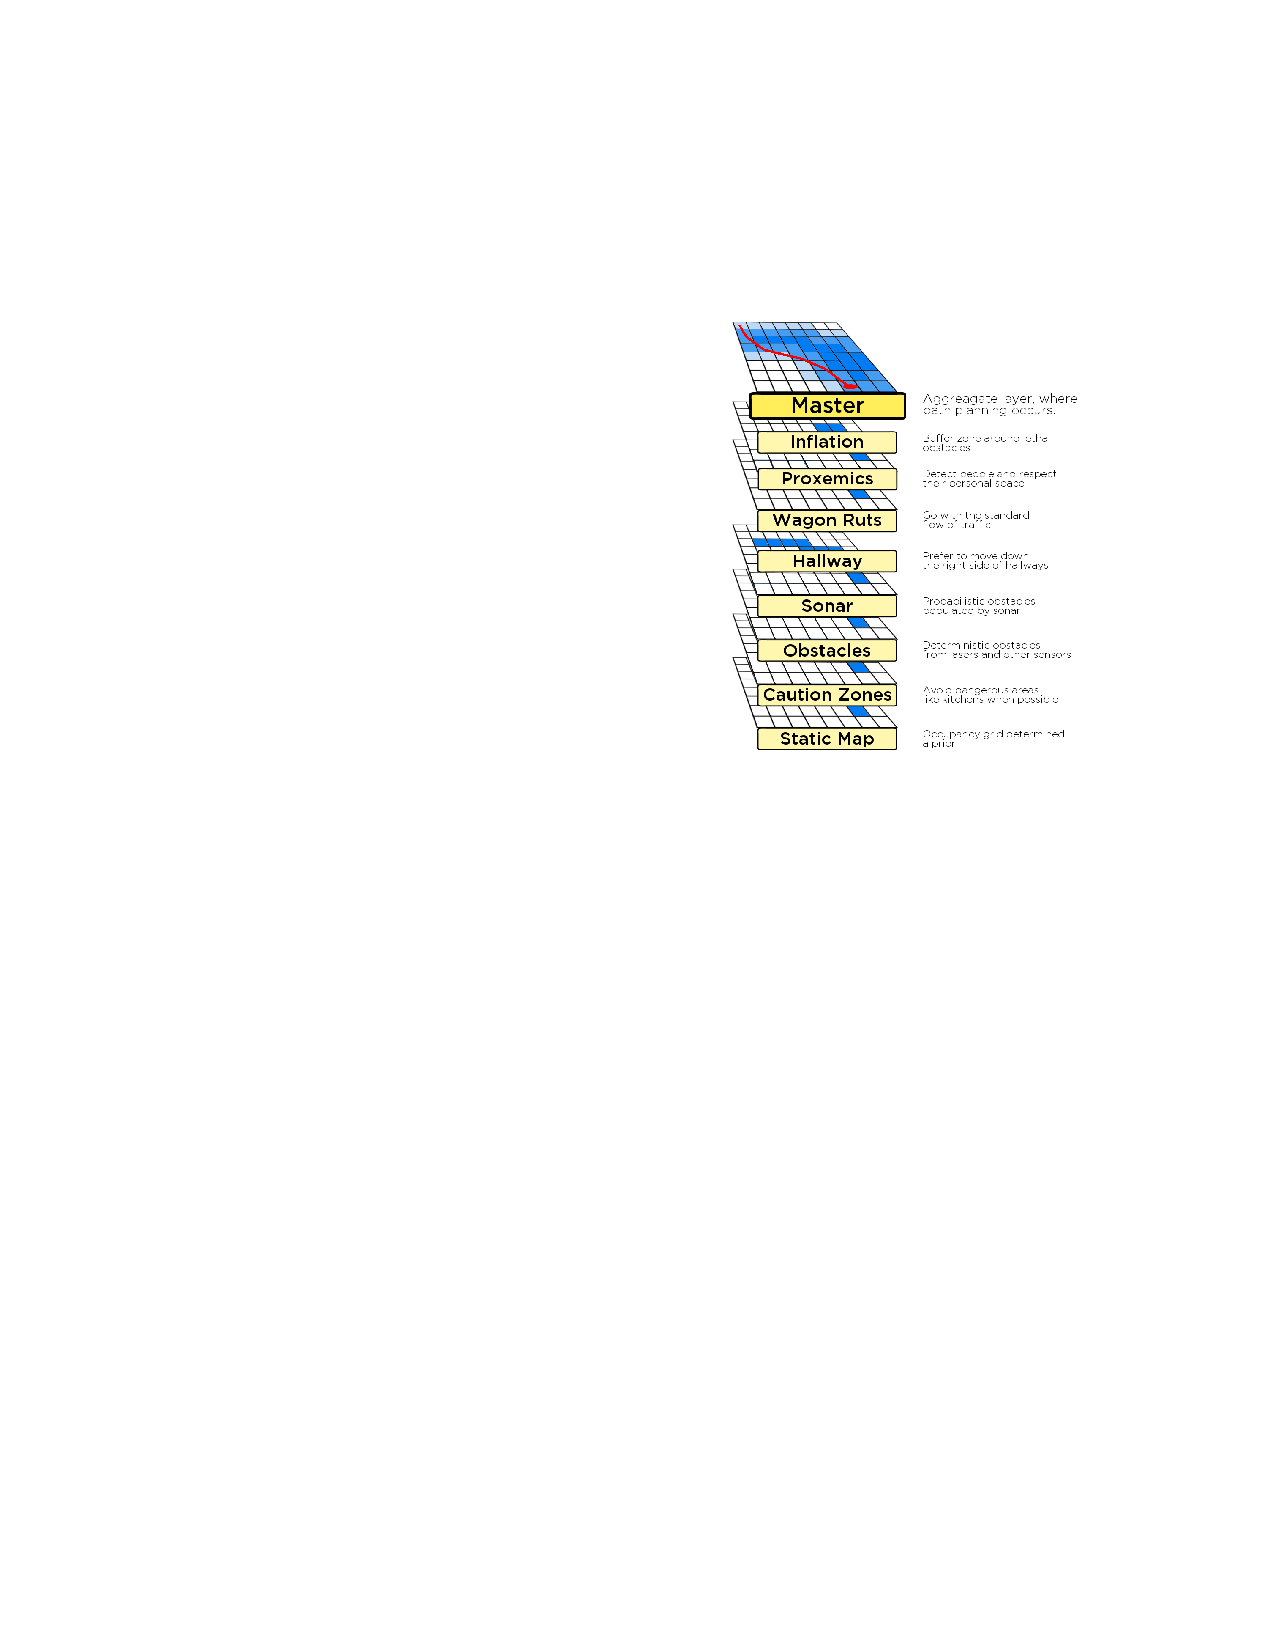
\includegraphics[width=0.45\linewidth]{layeredMaps}
	\caption{一组costmap图层,展示了使用分层costmap方法可实现的不同上下文行为。}
	\label{fig:costMap:layers}
\end{figure}

\section{相关工作}\label{sec:relatework}
这项工作的重点是适用于规划路径的地图的网格表示方式。 
20世纪80年代,由Moravec及其合作者在卡内基梅隆大学(CMU)开发的占据网格(occupancy grid)是现代代价地图鼻祖\cite{matthies1988integration,moravec1989sensor}。 
占据网格的语义值很直观:每个单元格的值表示该单元格存在障碍物的概率,因此其更新过程是贝叶斯规则的直接应用。 
Konolige\cite{konolige1997improved}和Thrun\cite{thrun2001learning}改进了概率模型,以便更好地定位障碍物。
基于网格的代价地图表示方法(其中网格值表示的不是概率而是通行代价)被证明是很实用的方法,尤其是当障碍物的位置是固定不定的情况下(不使用声纳探测仪)。
过去,代价地图主要是二进制的,单元格要么是被占据状态(occupied),要么是自由(free)状态。
现在的情况是,随着将更多的复杂代价的值加入代价地图,必然导致代价地图的语义信息过于混乱。
对于那些非致命的(non-lethal)代价值,即值介于occupied与free中间,通常表示软约束(soft constraints)。
自主驾驶车辆采用这样的值进行优化,从而能在街道上正确的一边进行行驶或采取其他优先驾驶行为\cite{ferguson2008efficiently}。
Gerkey和Agrawal\cite{gerkey2008break}在代价图中用不同的代价值表示不同类型的地形及其通行性。
软约束也可用于基于人机交互的约束。 
Sisbot等人的Costmap系统\cite{sisbot2007human}就考虑到个人的活动空间和视野,
而Kirby等人\cite{kirby2009companion}等人则对人在路的右边行走行为进行了建模。
Svenstrup等人\cite{svenstrup2009pose}、Scandolo和Fraichard\cite{scandolo2011anthropomorphic}开发了更为复杂为感知人类行为的导航代价计算方法。


\section{单源代价地图 (Monolithic Costmap)}
\label{sec:mono-costmap}

单源代价地图 (Monolithic Costmap), 所有数据皆存储于单个网格中,是当前工程实现costmap的基础,包括普遍使用的ROS\cite{quigley2009ros}。
本文着重于ROS功能包的算法及其实现,这是因为ROS已获得大量使用,运行于上十种机器人硬件上\footnote{\url{http://wiki.ros.org/navigation/RobotsUsingNavStack}}。
ROS使用一张单源代价地图进行全局规划,同时在局部规划中使用另一张单源代价地图进行规划。

单源代价地图被证实在规划最短无碰撞路径(collision-free path)方面是非常有效的。将初值写入代价地图的做法非常直观,但由于存储空间非常有限,更新过程存在问题,这就限制了它所能实现的功能类型非常有限、代价地图的利用效率不高、可扩展性不强等缺陷。单源代价地图的主要缺点如下:

\emph{\color{blue}1) 更新期间的信息很有限}:单源代价地图的一个很大的缺陷是代价地图中的大部分信息存储于一个位置。考虑一个简单的传感器数据与全局代价地图中已有值之间冲突的例子。传感器数据表明地图中的某个区域是开阔的,而代价地图上却说明该区域存在障碍。更新代价地图的正确方法应与数据的来源及附加的语义信息有关。一种情况是先前的值是已经移动的人的位置;所以,正确的处理方式是将代价图中标记为“lethal”(致命区域)的值更新为“free”(自由区域),使得机器人可以在新腾出的空间通行。但是,一个同等有效的情况是:代价地图中的值来自静态地图的值,静态地图在创建的时候就包含了传感器无法看到的障碍物,例如玻璃墙。此种情况下,代价地图中应保留“lethal”值。

在单源代价地图中是无法区分这两种情况的,因为两种情况都在代价地图中将它标记为“lethal”。只要代价地图中的值为单种类型值,代价地图就会从数据中删除代价地图所表示的任何语义信息。

%This is also problematic for properly handling three-dimensional obstacle data. The original developers of the ROS implementation encountered this problem when they used three-dimensional sensors like a tilting laser range finder. If the obstacle data is stored only in the monolithic costmap, obstacles at different heights could be inappropriately removed by clearing observations. Thus, they introduced voxel grids to keep track of the additional information[12]. The solution works for extending the mono
%lithic costmap’s functionality in this one use case, but does not generalize.

在单源代价地图正确处理三维障碍物的数据也是有问题的。ROS的早期开发人员在使用像倾斜的激光传感器这种三维传感器时也遇到该问题。假如障碍物数据仅存储在单源代价地图中,可通过清除观察来移除不同高度的障碍物。因此,他们引入了体素网络(voxel grids)以跟踪其他信息\cite{marder2010office}。这种解决方案适合在该用例中扩展单源代价地图的功能,但没有推广性。


%The limited information becomes more problematic as the number of data sources and types for the costmap increases. Consider when there are multiple non-lethal data sources, each with an individual semantic meaning. If the values are added together in the monolithic costmap, a change to one of the values will result in each of the individual values needing to be recalculated.

随着代价地图的数据源和类型的数量增加,这种有限信息的存储结构更成为问题。
考虑存在多个"non-lethal"(非致命区域)的数据源,每个数据源带有自己的语义信息。
如果在单源代价地图中将多个"non-lethal"的值简单相加,其中一个值发生变化将导致每个语义信息需要重新计算。


%2) Fixed Update Areas: The lack of semantic information in the monolithic costmap also makes it difficult to tell how long any particular cost value has been in the costmap. Hence, if the updated area needs post-processing or to be published to some external source, there is no established way to determine the scope of the most recent updates. An ineffective way to deal with this problem is to conservatively estimate a swath of the map that covers the entire area that could have been updated, which is what the ROS   plementation does. In practice this means updating a roughly 6m x 6m square around the robot, regardless of how much of that space was actually updated.

\emph{\color{blue}2)固定更新区域}:
单源代价地图缺少语义信息,很难判断代价图中任何特定代价的持续时间。 因此,如果更新的区域需要后处理(post-processing)或要发布到某些外部源,则没有确定的方法来确定最近更新的范围。 处理该问题的一种无效方法是保守估计覆盖整个区域的地图区域,这些区域可能已经更新,这是ROS的实现所要做的。 实际上,这意味着要在机器人周围更新大约 $6m \times 6m$的方形区域,无论实际更新了多少空间。

%2)固定更新区域:在整体成本地图中缺乏语义信息,也很难判断成本价值在成本地图上有多长时间。因此,如果更新的区域需要后处理或发布到一些外部源,就没有确定的方法来确定最近更新的范围。处理这个问题的一个无效的方法是保守地估计覆盖整个区域的地图,这些区域可能已经更新,这就是ROS的实现所做的。在实践中,这意味着要在机器人周围更新大约600万x 600平方的空间,不管这个空间实际上更新了多少。

%3) Ad-hoc Update Process: The lack of an established paradigm for maintaining and updating a costmap results in implementations that take an ad-hoc approach. This method has worked thus far due to the relatively small number of data sources used in practice, but it becomes infeasible as the number of sources increases. In order to ensure that the data is combined in the correct way, every data source needs to be aware of every other data source.

\emph{\color{blue}3)临时更新过程}:缺乏用于维护和更新代价地图的既定范例,导致只能采用临时的方法进行实现。 目前为止,由于实际使用的数据源数量相对较少,该方法已经奏效;但随着数据源数量的增加,这种方法也会变得不可行了。 为了确保以正确的方式组合数据,每个数据源都需要清晰了解其他数据源的使用过程。

%(3)临时更新过程:没有为如何添加不同的信息来源和组合来生成成本地图的设置范例。因此,即使语义问题已经被解决,信息源也会以特定的方式更新costmap。到目前为止,这种方法已经奏效,因为在实践中使用的数据源相对较少,但是随着源数量的增加,这种方法也变得不可行了。即使在以前的工作中,为计算成本定义了有用的算法,他们使用的过程实际上是不透明的。如果没有关于如何精确地更新成本地图的信息,复制结果就会变得更加困难。

%Even in the prior work that define useful algorithms for calculating costs, the process that they use to actually integrate them with their full costmap is usually opaque. Without the information about how precisely costmaps are updated, accurately replicating results becomes impossible.
即使在之前的工作中为计算成本定义了有用的算法,但它们与完整的代价地图进行集成的过程通常是不透明的。 如果没有关于如何更新代价地图的信息,则无法准确复制结果。


%4) Semantically Fixed Interpretation: In addition to limiting the amount of information that costmaps contain, monolithic costmaps also constrain the types of information that can be used. The monolithic costmap also only affords a single interpretation of the values in the costmap. The original occupancy grid definition of costmaps used a probabilistic interpretation. Alternatively, the value could represent some cost/penalty for being at a certain location. With the monolithic costmap, it is ambiguous how to combine a probabilistic data source with a cost-based one.
\emph{\color{blue}4)固定的语义解释}:除了限制代价地图包含的信息之外,单源代价地图还限制了可以使用的信息类型。 单源代价地图也只能对代价地图中的值进行单一解释。 代价地图的原始占用网格定义使用了概率解释。 即,该值表示在某个位置的代价/惩罚量。 对于单源代价地图,并没有明确定义如何将概率数据源与基于代价的数据源结合的方式。

%4)不灵活的配置:除了限制成本地图所包含的信息量外,单源成本地图还限制了可以使用的信息类型。这个约束来自于原占用网格定义的costmap,其中每个值只表示单元格中的一个障碍的概率。类似地,在价格为成本的网格中,输入到costmap的信息输入的类型仅限于成本。因此,如何将概率网格与基于成本的网格结合起来是不明确的。

%ROS costmap实现有额外的问题,因为它所接受的唯一类型的信息是二进制的障碍数据,即存在明显的障碍或者绝对自由空间。添加非致命成本并不适合其整体框架。在costmap中有一个数据类型,信息是语义固定的。
%
%

%The ROS costmap implementation has additional problems since the only type of information it accepts is binary obstacle data, i.e. where there are definitely obstacles or there is definitely free space. Adding non-lethal costs does not fit into its monolithic framework. With just one data-type in the costmap, the information is semantically fixed.
ROS的代价地图实现还有其他问题,因为它接受的唯一信息类型为是否二进制障碍数据,即要么存在明显的障碍,要么为绝对自由空间。 不适合在现有的框架上增加非致命(non-lethal)的代价属性。 因为costmap只有一种数据类型,所以语义信息是固定不变的。

%\subsection{限制}
%
%在计算最小长度的无碰撞路径时,单源代价地图已经被证明是有效的。然而,可实现功能的类型和成本地图的效率是有限制的。在整体成本地图上的局限性是,在代价图和它们的非结构化的更新方面缺乏信息.
%
%1) 在更新步骤中有限的信息:单源成本地图的主要限制之一是,costmap中的大多数信息存储在一个位置。这可以包括来自诸如静态映射和每个传感器的障碍信息,以及非致命成本和任何计划优化。将所有已编译的成本数据存储到这个简单的数据结构中,就会丢失关于它来自何处以及每个值表示什么的语义信息。由于不同数据源的相互混合,使得更新代价地图变得更加困难。一旦成为一个单一的代价地图,价值缺乏上下文。
%
%例如,传感器数据和静态映射引入的致命障碍之间没有区别。因此,当清除观测与致命障碍重叠时,就无法确定其来源。ROS实现假设,清除观察应该优先考虑,认为致命障碍是在静态代价地图中移动或错误的一个障碍。这
%
%策略可以在许多场景中运行,但也会导致问题。如果数据中存在噪声或定位不当,则静态墙会被错误地清除,从而导致机器人规划一条穿过墙壁的路径。实践经验显示,PR2机器人上的ROS导航系统已经证实了这种趋势,结果使机器人看起来相当不聪明,因为它常常试图通过开车到房间的一个角落,而没有门,试图离开房间。
%
%这个例子也有问题,它是基于视觉的传感器读数的长期记忆,即玻璃墙。如果所有的传感器数据都保存在单源代价地图中,那么就可以通过清除激光观测(包括玻璃障碍物)来清除标记的声纳障碍。因此,机器人可能会试图通过玻璃,这显然是次优的。
%
%另一个例子,膨胀过程也使更新过程复杂化。 由于不断变化的地区,必须在每个周期重新计算更新障碍物附近每个费用图单元格的膨胀值。 由于代价地图没有任何方法来确定代价地图中的值的来源,所以ROS实现会清除更新数据区域中的所有非致命值,然后使用更新的位置重新计算它们。 这掩盖了引入非致死值的任何其他数据源,并强制在每个周期重新计算这些值。
%
%第三个例子是遇到ROS实现的原始开发者,并涉及三维传感器。 如果数据仅存储在单源代价地图中,则通过清除观察值可能会不适当地删除不同高度的障碍物。 因此,他们引入了体素网格来跟踪附加信息。 但是,此修复仅适用于一种类型的数据,并且不能扩展到所有其他类型的数据。
%

\section{分层代价图}

\subsection{数据结构和更新算法}
%To counteract the limitations introduced in the previous section, we devised the layered costmap. The data structure still contains a two-dimensional grid of costs that is used for path planning. The key difference is how the values of this master costmap are populated. Instead of storing data directly in the grid, the layered costmap maintains an ordered list of layers, each of which tracks the data related to a specific functionality. The data for each of the layers is then accumulated into the master costmap, which takes two passes through the ordered list of layers.
%为了抵消前一节中介绍的限制,我们设计了分层成本地图。数据结构仍然包含用于路径规划的二维成本网格。关键的区别是如何填充这个主代价图的值。分层costmap不是直接在网格中存储数据,而是维护一个有序的层列表,每个层都跟踪与特定功能相关的数据。然后,将每个层的数据累积到主代价地图中,它需要两个遍历层的有序列表。

为了消除上一节中介绍的种种限制,我们设计了分层代价地图(layered costmap)。 数据结构仍包含用于路径规划的二维代价网格。 最重要的区别在于如何填充此主代价地图(master costmap)的值。 分层代价地图不是直接在网格中存储数据,而是维护有序的地层列表(layered list),每个层都跟踪与特定功能相关的数据。 然后将每层的数据累积到master costmap中,这需要在有序的layered list进行两次遍历。

%In the first pass, the updateBounds method, each layer is polled to determine how much of the costmap it needs to update. The layers are iterated over, in order, providing each layer with the bounding box that the previous layers need to update (initially an empty box). Each layer can expand the bounding box as necessary. This first pass results in a bounding box that determines how much of the master costmap needs to be updated. During the second pass, the updateValues method is called, during which each successive layer will update the values within the bounding box’s area of the master costmap. Fig. 2 illustrates the update algorithm using a set of layers that replicate the behavior of a basic monolithic costmap.
%在第一个传递中,updateBounds方法,每个层被轮询,以计算它需要更新多少成本地图。顺序遍历,依次为每个层提供前层需要更新的边界框(最初是一个空框)。该层可以根据需要扩展边框。第一个传递的结果是一个边界框,它决定了需要更新多少主代价地图。在第二个传递过程中,调用updateValues方法,在此期间,每一个连续层将更新主costmap的边框区域内的值。图2使用一组复制基本单块代价地图的行为的层来说明更新算法。

在第一次遍历中,即\mintinline{c++}{updateBounds}方法中,每个层都被轮询以确定代价地图的更新量。 按顺序遍历各层,依次为每层提供前一层需要更新的边框(最初为空框)。 每层都可以根据需要扩展边框。 第一次遍历会生成一个边框,用于确定master costmap需要的更新量。 第二次遍历将调用\mintinline{c++}{updateValues}方法,在此期间,每个连续层将更新master costmap的边框区域内的值。 图\ref{fig:costMap:updateAlg}展示了使用一组基本代价地图进行的复制行为来说明更新算法。

\begin{figure}[!htb]
	\centering
	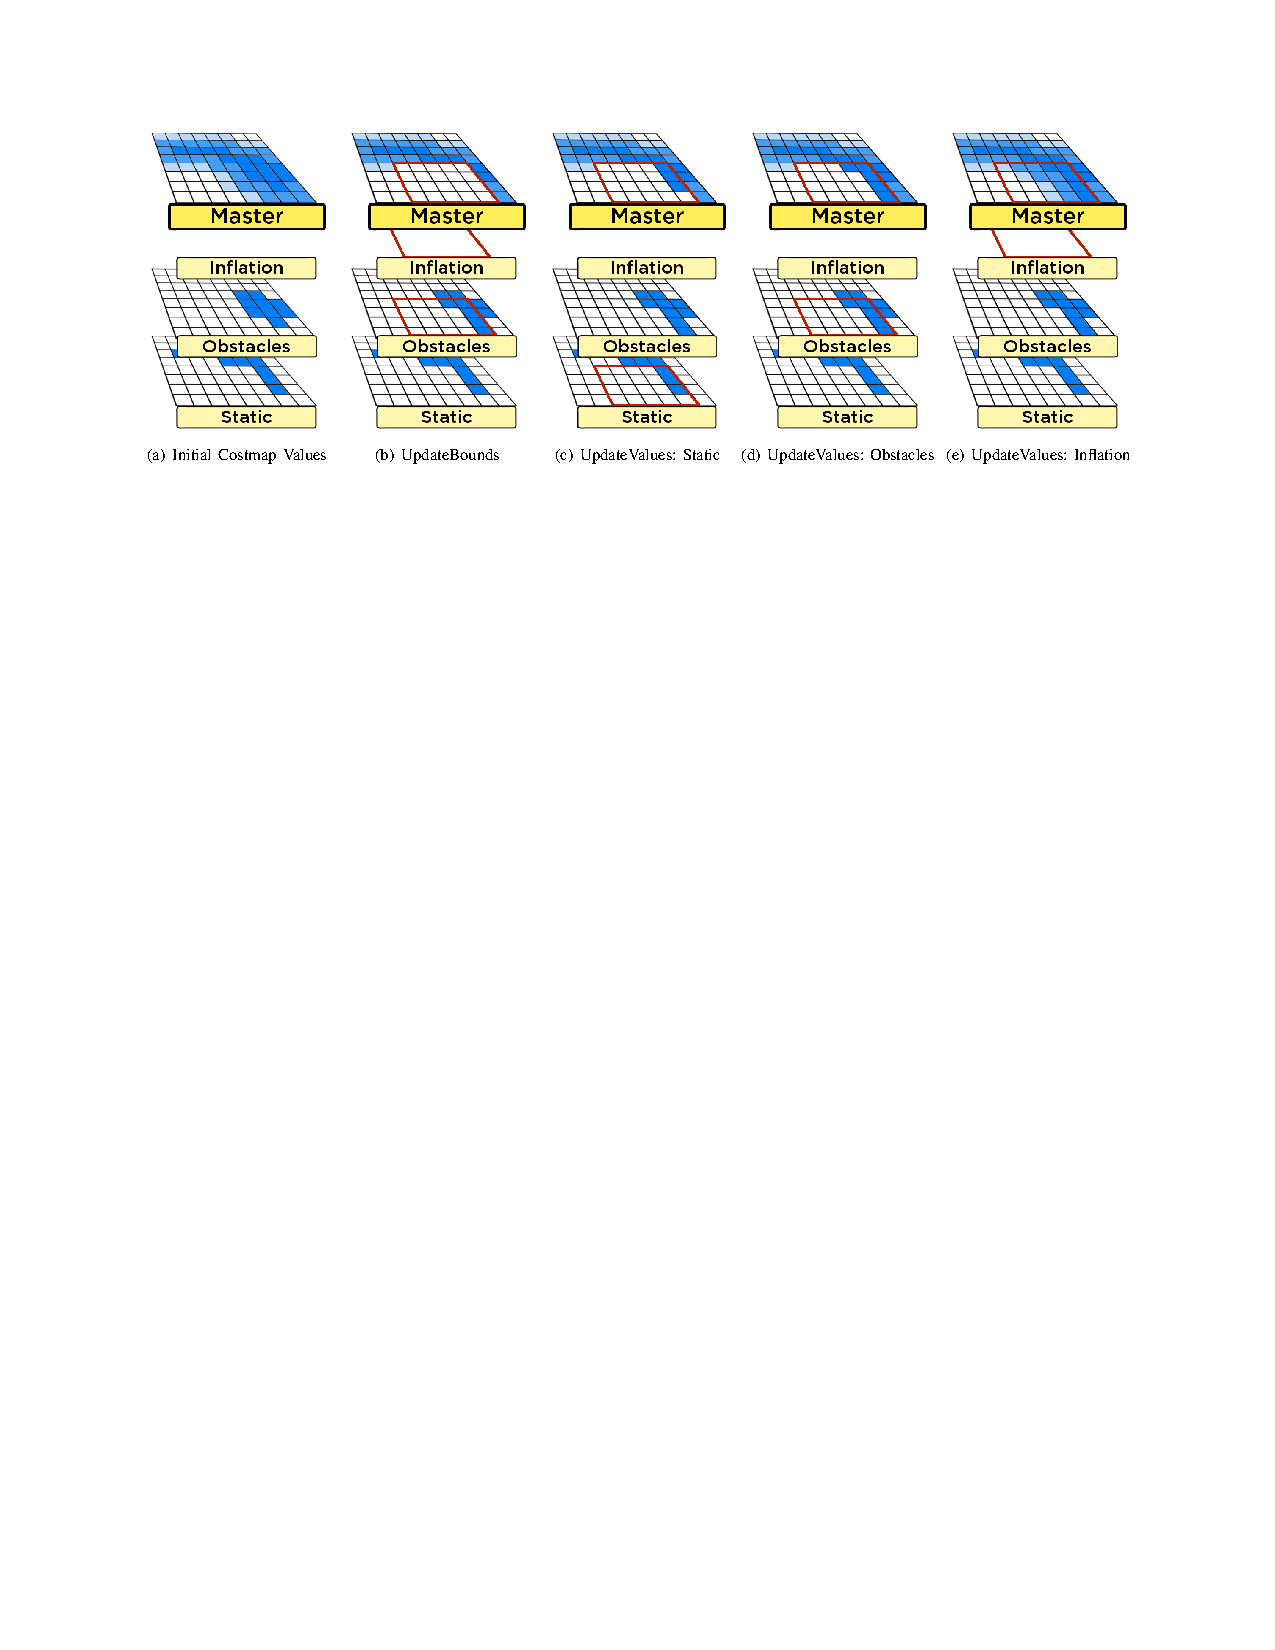
\includegraphics[width=\linewidth]{AlgUpdate}
	\caption{更新算法。(a)中,分层costmap由三个功能层和一个master costmap组成。 障碍物层和静态层保留有自己层的网格副本,而膨胀层没有。 为更新costmap,算法首先在每个图层上调用\mintinline{c++}{updateBounds}方法 (b),从有序列表中的第一个图层开始(显示在底部)。 为了确定新更新区域的边界,障碍层根据传感器的新数据更新自己的costmap。 结果为一个每层都需要更新的区域的边框。 接下来,每个层依次调用\mintinline{c++}{updateValues}方法更新master costmap中的边框区域,从静态层(c)开始,然后是障碍层(d)和膨胀层(e)。}
	\label{fig:costMap:updateAlg}
\end{figure}
%更新算法——在(a)中,分层的代价地图有三层和主代价地图。障碍和静态层保留了它们自己的网格副本,而膨胀层则没有。为了更新costmap,算法首先调用每个层上的update界限方法(b),从列表的第一层开始,显示在底部。为了确定新的边界,障碍层用新的传感器数据更新自己的成本地图。结果是一个包含每个层需要更新的所有区域的边界框。接下来,每一层依次使用updateValues方法更新边界框中的master costmap,从静态层(c)开始,然后是障碍层(d)和膨胀层(e)
%Update Algorithm - In (a), the layered costmap has three layers and the master costmap. The obstacles and static layers maintain their own copies of the grid, while the inflation layer does not. To update the costmap, the algorithm first calls the updateBounds method (b) on each layer, starting with the first layer in the ordered list, shown on the bottom. To determine the new bounds, the obstacles layer updates its own costmap with new sensor data. The result is a bounding box that contains all the areas that each layer needs to update. Next, each layer in turn updates the master costmap in the bounding box using the updateValues method, starting with the static layer (c), followed by the obstacles layer (d) and the inflation layer (e).


%Some layers will maintain their own version of the costmap for caching results. This is one of the primary ways the data structure maintains semantic information about the data. For example, an obstacles layer keeps a private costmap of the same size as the master costmap to store the results of all previous ray-tracing and marking steps. Since the values in the private costmap are only accessible to the particular layer, the information stored within cannot be lost by another data source writing over it. This in turn minimizes how frequently the costmap must recalculate values that had previously been overwritten.
%
%有些层将维护自己的全尺寸版本的costmap缓存结果。这是数据结构维护关于数据的语义信息的主要方式之一。例如,一个障碍层保存了一个私有的costmap副本,用于存储之前所有的射线跟踪和标记步骤的结果,而不是每次都重新计算它们。但是,由于这些成本都保存在私有代价地图中,因此,这一层不可能意外地覆盖不必要的数据。

某些图层会维护自己版本的costmap用于缓存结果。 这是数据结构维护语义信息的主要方式之一。 例如,障碍层保留与master costmap相同大小的私有costmap,以存储所有光线跟踪(ray-tracing)和标记步骤的结果。 由于私有costmap中的值只能由特定层访问,因此存储在其中的信息不会因为其他数据源的写入操作而丢失。 
反而最小化了costmap由于先前被覆盖写入新值而必须重新计算的频率。

%Other layers do not require that much data to be kept from cycle to cycle and will update the master costmap with their data on each turn, or will simply operate on the data that other layers have already written into the master costmap.
%其他层不需要将大量数据从循环中保存到循环,并且将在每个回合中更新主代价地图,或者简单地操作其他层已经写入了master costmap的数据。
其他层不需要在循环之间保留太多数据,并且将在每个回合中使用其数据更新master costmap,或者仅对其他层已经写入master costmap的数据进行操作。

%The example in Fig. 2 shows how the previous ad hoc approach used to generate the costmap can be refined into a neat, well-defined process. A more precise explanation of how each layer changes the master costmap is in section VI.
%图2中的示例展示了以前用于生成costmap的特定方法可以被细化为一个整洁的、定义良好的过程。在边界更新步骤中,静态映射通常不需要更新边界框,因为根据定义,什么都没有改变。它只会在收到地图后立即更新边界框,以便将整个地图加载到主代价地图中。障碍层将在updateBounds传递过程中处理所有新的传感器数据,以确定其空间范围,并相应地更新边界框。这意味着updateValues传递将花费更少的时间在障碍层,因为它只需要将存储在层网格中的值与主网格中已经存在的值进行比较。在默认配置中,障碍层将选择两个值的最大值。

图\ref{fig:costMap:updateAlg}中的例子展示以前用于生成costmap的具体操作方法(ad hoc approach)如何被细化为一个整洁、良好定义的过程。 
关于每层如何改变master costmap的详细说明,请参照第\ref{sec:layers}节。


\subsection{优点}
%The layered costmap approach specifically addresses the
%limitations of the monolithic costmap.
分层代价地图方法显然解决了单源代价地图的局限性。

%1) Clearer Update Step: Different types of costmap information are added to separate layers in the layered costmap approach, making the update step more clearly delineated. If the desired behavior included the ability to treat static obstacles, sensed laser obstacles and sensed sonar obstacles differently, storing those obstacles in their own layers simplifies the bookkeeping substantially. Each layer only needs to keep the information consistent with other information of the same type.
%1)更清晰的更新步骤:将不同类型的代价地图信息添加到分层的costmap方法中,使更新步骤更加容易。如果想要的行为包括治疗静态障碍、感知激光障碍和感知声纳障碍的能力,将这些障碍存储在自己的图层中,可以大大简化簿写操作。每个层只需要保持与相同类型的其他信息相一致的信息,而不是先前的方法。
\emph{\color{blue}1)更清晰的更新步骤}:在分层的代价地图方法中,不同类型的代价地图信息添加到单独的层中,使得更新步骤更为清晰。 如果希望将静态障碍物、从激光检测到的障碍物、及从声纳检测到的障碍物区别处理,则将这些障碍物存储在各自的层中显然简化了信息的记录方式。 每层只需要保持同类型的信息一致即可。

%The layered costmap also eliminates contention between the competing costmap information sources. Each layer only needs to be updated as new information of that type comes in. If a layer remains largely static, it does not need to be recalculated each time another layer updates some subarea. The static layer merely needs to update into the master costmap and the update can move on to the next layer.
%分层代价图也消除了竞争代价图信息源之间的争用。考虑一下有一个软约束层来编码代理信息和膨胀层。在单岩性的实现中,这两种类型的信息都将存储在奇异的代价图中。当需要重新计算通胀值时,所有非致命值都需要清除,包括来自代理约束的值。如果代理信息更新的频率低于整个代价地图,单源代价地图需要从每个周期的代理层重新计算值。使用分层的代价地图,代理层不需要在每次通货膨胀的时候清除和重新计算。相反,它只会将其值复制到主代价地图,这是一个非常快的过程。
分层的代价地图还消除了同源代价信息之间的争用。 每层只需在插入同类型的新信息时更新。如果一个层保有很大的静态区域,则另一个层在更新某个子区域时无需重新计算。 静态层只需要更新到主代价地图,然后更新可以移到下一层。

%This clearer separation of concerns also makes the individual components of the costmap easier to tune. Initial users can introduce one layer at a time and debug each in turn.
%​ 这种更清晰的关注点分离也使得代价地图的个人组成部分更容易调整。初始用户可以一次引入一层,然后依次调试。
这种更清晰的关注点分离技术使得各个代价地图组件更容易调整。 初始用户可以一次只引入一个层,并依次调试每层。

%​2) Dynamic Update Areas: As opposed to the fixed or unknown regions that are updated on each round of updates in the monolithic costmaps, by virtue of the updateBounds pass through the layers, the layered costmap only updates the region of the map that the individual layers deem necessary. This gives the costmap extra stability, guaranteeing that only values within the bounding box are updated. Furthermore, it can potentially be more efficient by updating smaller amounts of the map. 
%2)动态更新区域:相对于固定的或不知道的区域,在单源成本地图上的每一轮更新中更新的区域,通过层间的updateBounds,分层代价图只更新了单个层认为需要的映射区域。这给了costmap额外的稳定性,确保只更新了边框内的值。此外,通过更新更小的地图,它可能更有效。
\emph{\color{blue}2) 区域动态更新}:与单源代价地图中每一轮更新中更新固定区域或更新未知区域相反,由于updateBounds通过图层传递,分层代价地图仅更新各个图层认为需要更新的区域。 这为costmap提供了额外的稳定性,保证只更新边界框内的值。 此外,更新量较小的地图可能更有效。


%3) Ordered Update Process: As opposed to the undefined order in which elements in the monolithic costmap were updated, the layered costmap has an explicit ordering. In our example, it is clear that the inflation layer will inflate values from both the obstacles and static layers by virtue of the inflation layer coming after the other two in the ordered list. Furthermore, the interactions between layers are explicitly specified. Each costmap can be configured to combine the previous value and the layer’s value as a maximum, minimum or some other mathematical function of the two.

\emph{\color{blue}3) 有序更新}:与单源代价地图未定义单元格的更新顺序相反,分层代价地图具有显式有序的特点。 在我们的例子中,显然,膨胀层膨胀的是障碍物层和静态层的值,因为膨胀层在有序表中是排在后两者之后的。 此外,层之间的交互是显式指定的。每个costmap可以配置为将前一个值和层的值合并为最大值、最小值或以两者为输入的的其他数学函数。

%4) Flexible Configurations: Finally, and most importantly, the capabilities of the layered costmap approach are endless. The layers needed to implement an equivalent set of behaviors to the previous implementation are only the beginning. As many layers as the robot operator desires can be added  to the layered costmap. The result is that the individual layers can implement arbitrarily complex logic for updating the costmap, expanding the costmap’s semantic possibilities. Each of the layers can also have its own independent representations of the data, such that probabilistic occupancy grids can exist in their own layers alongside cost-based layers.
%​ 4)灵活配置:最后,也是最重要的,分层成本地图方法的能力实际上是无限的。要实现与之前的实现等效的行为集所需的层仅仅是开始。机器人操作者的许多层都可以添加到分层的代价地图中。结果是,单个层可以实现任意复杂的逻辑来更新代价地图,扩展代价地图语义的可能性。正如我们在以后的个人层面讨论中所看到的,costmap可以包括概率层和非致命层,以及二进制障碍数据。

\emph{\color{blue}4) 灵活配置}:最后,也最重要的,分层代价地图方法的功能是无限的。 实现与先前实现的等效行为所需定义的层仅仅是个开始。 
可以将机器人操作员所需的多个层添加到分层代价地图中。 结果是,各个层可以实现任意复杂的逻辑来更新代价地图,从而扩展了代价地图的语义可能性。 每个层还可以独立具有自己的数据表示方式,使得概率占据网格可以与基于代价的层一起存在于它们自己的层中。

\section{对比}

\subsection{实现细节}
%Although the algorithm and data structure for layered costmaps are system-agnostic, due to the ubiquity of the  platform, we focused on implementing the system to work with the ROS Navigation stack in order to demonstrate the capabilities of the approach. The layered costmap implementation keeps the costmap 2d API mostly in tact and like the rest of the navigation code, is implemented in C++, as are each of the layers.
%虽然分层代价地图的算法和数据结构是系统无关的,但由于平台的普遍存在,我们将重点放在实现系统与ROS导航堆栈一起工作,以演示方法的能力。分层的costmap实现使得costmap 2d API大部分都是在触觉中,和其他的导航代码一样,是在c++中实现的,每个层都是这样。
尽管分层代价地图的算法和数据结构与系统无关,但由于平台的普遍性,我们将重点实现系统与ROS导航功能包以演示该方法的功能。 分层代价地图的实现使得costmap 2d的API保持较好的通用性,与导航功能的其他代码一样,采用C++实现;每层皆如此。

%Implementing a layer is quite easy. First, a new class must be created which extends the costmap 2d::Layer class. This means implementing the initialize function (where the layer can independently subscribe to any data sources in the ROS ecosystem), the updateBounds
%function and the updateCosts function. Independently compiled layers can be plugged in to the layered costmap with simple run-time parameter changes.
%​ 实现一个层很容易。首先,必须创建一个扩展costmap 2d::层类的新类。这意味着实现初始化函数(该层可以独立地订阅ROS生态系统中的任何数据源)、updateBounds函数(更新上面描述的边界框)和updateCosts函数(将值写入到master costmap)。独立编译的层可以通过简单的运行时参数变化插入分层的代价地图。
工程化实现层非常简单。 首先,创建一个新类,它继承自\mintinline{c++}{costmap 2d::Layer}类。 这意味着需要实现初始化函数(其中层可以独立订阅ROS生态系统中的任何数据源)、\mintinline{c++}{updateBounds}函数(更新边框)、和\mintinline{c++}{updateCosts}函数(将值写入到master costmap中)。 
可以使用简单的运行时参数更改方法将独立编译的图层插入到分层的costmap中。
单独编译的层可以在运行时更改参数后以插件形式插入到分层代价地图执行。

%Whereas previously the costmap class had special cases to deal with whether there was a static map or not, or whether to track the obstacles in three dimensions, these cases are instead handled by configuring the global and local costmaps with different layers.
%​ 为了复制所有的功能,只有四种类型的层是需要的。之前,costmap类有特殊的情况来处理是否存在静态映射,或者是否在三维空间中跟踪这些障碍,分层的costmap被配置为不同的层。如图2所示,全球代价地图被复制到一个静态的地图层,一个障碍层和一个通货膨胀层。通过更改单个参数,可以将障碍层转换为voxel层。本地代价地图更简单,只是需要一个障碍或voxel层和一个通货膨胀层。
在分层代价地图之前,costmap类在处理是否存在静态地图、或者是否启用三维跟踪障碍物这些不同的情况时,是把它们作为特殊情况处理的。现在的做法变成了对全局代价地图和局部代价地图配置不同类型的图层来进行处理。

%The two implementations of costmaps were run through repeated simulated trials in Gazebo scenarios. The robot employed was the PR2, as was used in the initial benchmarking of ROS navigation[12]. After hundreds of simulations, we found no noticeable difference between the paths generated by the two implementations, with regard to path length, time to completion and relation to obstacles.
%​ 然后,在Gazebo场景中,通过重复的模拟试验,运行了两个代价映射的实现。使用的机器人是PR2,如在ROS导航的初始基准测试中使用的.Marder-Eppstein等人[12]。经过数百次模拟,我们发现,在路径长度、完成时间和与障碍物的关系方面,两种不同的方法产生的路径之间没有明显的差异。

我们在Gazebo的重复模拟试验中运行两种代价地图。 正如ROS导航功能包的基准测试采用的评估那样\cite{marder2010office},在PR2机器人上测试。 
经数百次模拟试验,我们发现两种实现方式生成的路径在路径长度、完成时间、及与障碍物的关系方面并没有明显差异。

\subsection{时间对比}
%One of the most critical statistics we analyzed was the average runtime of the costmap update cycle. Due to the speeds at which the local planning needs to run and adjust to new obstacles, the update process must be quite quick. The standard we aimed to achieve was an update frequency of at least 5 Hz (as had been used by the previous implementation), capping the individual cycle runtime at 0.2 seconds. The monolithic costmap was able to exceed that by an order of magnitude or two, depending on the specifics of the environment and the system running the costmap. The layered costmap implementation also depends on these variables. Ultimately, the layered implementation runs faster in certain scenarios and slower in a few corner cases.
%我们分析的最重要的统计数据之一是costmap更新周期的平均运行时。由于本地计划需要运行和适应新的障碍的速度,更新过程必须非常快。我们要达到的标准(如之前的实现所使用的标准)是至少5赫兹的更新频率,以0.2秒的时间限制单个的循环运行时。根据环境的具体情况和运行costmap的系统,单源成本地图的数量可以超过这个数字的两倍。分层的costmap实现也依赖于这些变量。最终,分层的实现在某些场景中运行得更快,在一些角落的情况下会更慢。
统计分析中最重要的数据指标之一是costmap的更新周期的平均运行时间。 由于局部规划需要根据运行速度和新出现的障碍物的情况调整速度,所以更新过程必须非常快。 需要达到的标准是至少5 Hz的更新频率(和前面的实现采用的一致),将单个周期的运行时间限制在0.2秒内。 根据环境的细节和运行代价地图的系统,使用单源代价地图的方法能够超过一个量级或两个量级。 毕竟分层的costmap实现也依赖于这些变量。 总之,基于分层思想的实现在某些情况下运行得很快,仅在极少数情况下运行速度变慢。

%In our simulations, the average update times for the global costmap were 0.00166 and 0.00236 seconds for the monolithic  and layered implementations respectively, and for the local costmap, the update times were 0.00493 and 0.00463 seconds respectively. Using a one-sided t-test, we found no significant difference in the average local update time. The global update time is significantly slower with the layered costmap (p<0.001). However, we determined that this was the result of a sparse simulated environment. In those simulations, the robot was placed in a completely open environment except for a single, relatively small obstacle between the robot and its goal. Thus, the robot’s laser readings extend to their maximal distances in most directions, resulting in a large area that the layered implementation needs to update.This area needs to be updated by each layer, slowing down the overall update speed.
%在我们的模拟中,全局代价图的平均更新时间分别为0.00166和0.00236,而对于本地代价图,更新时间分别为0.00493和0.00463。使用单边t测试,我们发现在平均本地更新时间上没有显著的差异。全球更新时间与分层成本地图(p< 0.001)显著地慢。但是,我们确定这是一个稀疏模拟环境的结果。在这些模拟中,机器人被放置在一个完全开放的环境中,除了一个单独的、相对较小的机器人和它的目标之间的障碍物。因此,机器人的激光读数在大多数方向上延伸至最大距离,从而产生一个分层的实现需要更新的大范围。这个区域需要被每一层更新,从而减慢整个更新速度

模拟实验中,在单源实现和分层实现这两种情况下,全局代价地图的平均更新时间分别为0.00166秒和0.00236秒;而局部代价地图的更新时间分别为0.00493秒和0.00463秒。 使用单边$t$-检验,我们发现局部规划的平均更新时间没有显着差异。 
在采用分层costmap实现时,全局规划的更新时间明显变慢($p<0.001$) 。
但是,我们确信这是稀疏模拟环境带来的问题。 
在这种模拟中,机器人被置于完全开放的环境,
而不是一个单独的、机器人与目标点存在一个相对较小障碍物的环境。
因此,机器人的激光读数在多数方向上会延伸到激光所能探测的最大距离,
这会导致各地图层实现需要更新一个很大的区域。
每一地图层都需要更新该区域,从而降低整体更新速度。

\begin{figure}[!htb]
	\centering
	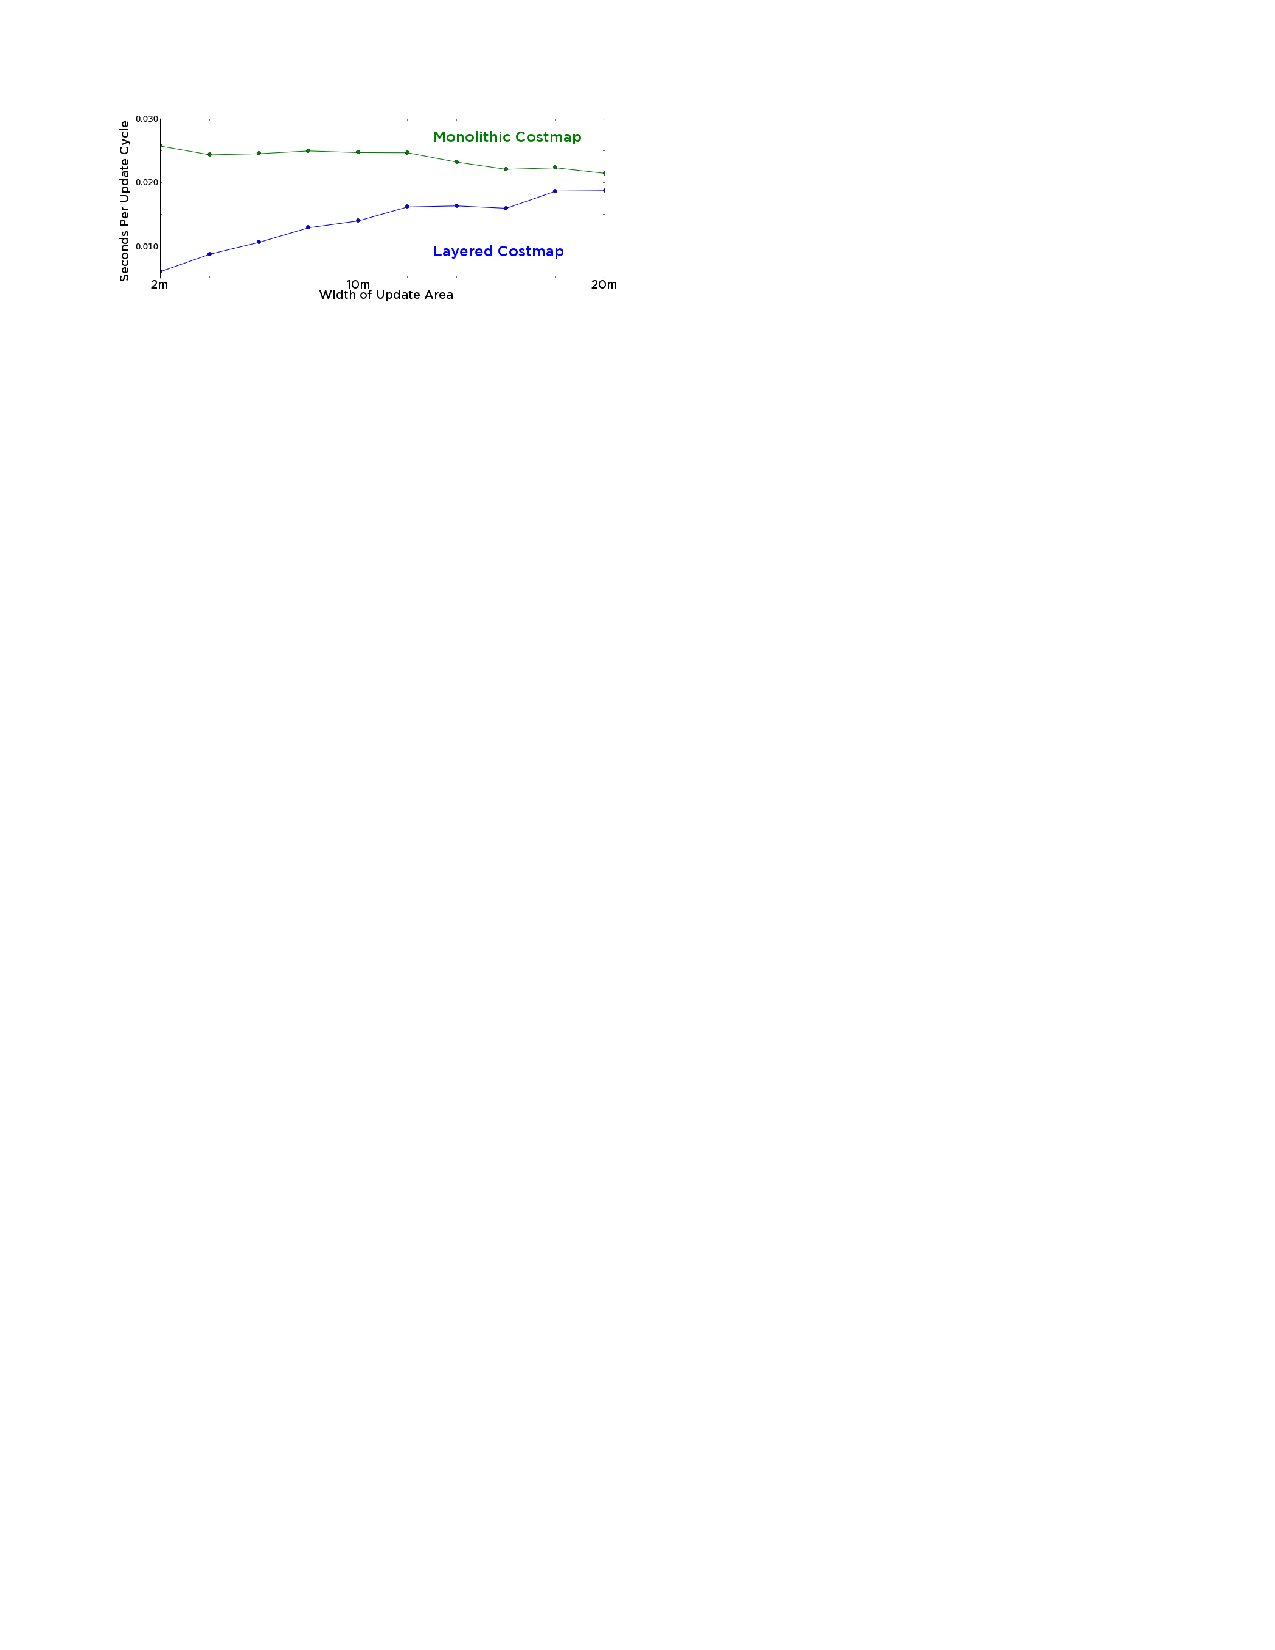
\includegraphics[width=\linewidth]{update-time-area}
	\caption{更新时间vs.更新区域 - 在单源实现的版本中,过程中更新区域大小保持不变,因而计时大致一致。在分层的实现版本中,更新区域会变化,因而计时上也会发生变化。}
	\label{fig:costMap:update-time-area}
\end{figure}
%Update Time vs. Update Area - Since the size of the updated area stays constant with the monolithic implementation, the timing stays roughly constant. However, the updated area varies with the layered costmap implementation, so the timing changes as well.

%We also simulated the robot in more cluttered environments, in which the robot was surrounded on all sides by walls at set distances away. With walls very close to the robot, the update area is much smaller. As seen in Fig. 3, in this scenario, the layered costmap is faster. As the updated area grows, the monolithic implementation’s update time stays roughly constant, whereas the layered costmap’s update time grows to match the increasing number of cells to update. Given that the costmap system is designed for working in cluttered, fast-changing environments, the layered costmap’s speed in those environments are more relevant.
%​ 我们还在更混乱的环境中模拟了机器人,机器人在各个地方被墙壁环绕。由于墙壁非常接近机器人,更新区域要小得多。如图3所示,在这个场景中,分层代价地图更快。随着更新区域的增长,整体实现的更新时间基本保持不变,而分层的costmap的更新时间会增加,以匹配更新的单元格数量。考虑到costmap系统是为在混乱的快速变化的环境中工作而设计的,在这些环境中分层的costmap的速度更有意义。
我们还在一个比较絮乱的模拟环境对机器人作了测试\footnote{译者注:絮乱区域是相对于平坦、开阔区域而言},其中机器人的所有侧面都被一定距离的墙所包围。 由于墙壁与机器人很近,因此需要更新的区域要小得多。 
如图\ref{fig:costMap:update-time-area}所示,在这种情况下,分层的代价地图方法更快。 随着更新区域的增长,单源版本的更新时间大致保持不变,而分层版本的更新时间会增长以匹配更新的单元格数量发生增加的现实情况。 
%鉴于costmap系统专为在混乱,快速变化的环境中工作而设计,分层costmap在这些环境中的速度更具相关性。
鉴于代价系统的设计多用于絮乱、快速变化的环境,分层代价在这些环境中的速度表现与实际情况较为吻合。

\subsection{在真实世界中导航}
%In addition to our thorough simulated tests, we also tested the layered costmap on the PR2 platform in the real environments. The tests were primarily performed in the office environment at Willow Garage. Using the layers to mimic the monolithic costmap structure, the PR2 was able to successfully replicate all the path planning behavior of the previous implementation. However, the more exciting results occurred when we modified the layers to get behavior that was impossible with the monolithic costmaps.
%除了完整的模拟测试之外,我们还在实际环境中测试了PR2平台上的分层代价地图。这些测试主要是在车库的办公室环境中进行的。通过使用这些层来模拟整体的costmap结构,PR2能够成功地复制以前实现的所有路径规划行为。然而,当我们修改层来获取不可能的单源代价地图时,会出现更令人兴奋的结果。
除了模拟测试外,我们还在真实环境中用PR2平台测试了分层代价地图的性能。 
测试地点主要在Willow Garage的办公环境中进行。 
使用地图层来模拟单源的costmap结构,能够让PR2成功复现先前实现的所有路径规划行为。 
但是,当我们修改地图子层以提取使用单源代价地图无法实现的行为时,产生了激动人心的结果。

%First, by separating the static and obstacle layers, we controlled whether the obstacle layer had the power to overwrite the static map. As mentioned in section III, the monolithic costmap navigation could improperly clear parts of the static map, leading to the robot planning a path that moved through a solid wall. By only allowing the obstacle layer to ray-trace and clear the sensed obstacles (and not those in the static map), the wall never was cleared from the master costmap, eliminating the embarrassing wall-charging behavior. 
%首先,通过分离静态和障碍层,我们可以控制障碍层是否有能力覆盖静态映射。如第二节所述。一个整体的costmap导航可以不正确地清除静态映射的部分,导致机器人规划一条穿过坚实墙的路径。通过只允许障碍物层到射线追踪和清除感知障碍(而不是静态地图上的障碍物),这堵墙从来没有从主代价地图中清除,消除了令人尴尬的穿墙行为。
首先,通过分离静态层(static layers)和障碍层(obstacle layers),我们测试障碍层是否具有覆盖静态地图的功能。 
正如第\ref{sec:mono-costmap}节所述,使用单源代价地图进行导航的一个问题是可能会错误清除静态地图的某些部分,导致机器人规划出一条穿过实心墙的路径。 
仅通过允许障碍物层进行光线跟踪并清除检测到的障碍物(不是静态地图上的障碍物),墙从未在主代价地图中被清除,这就消除了令人尴尬的穿墙通行行为。

%The introduction of new layers also enables new previously impossible behavior. The  motivating use case behind our investigations of the costmap was to create sociallyaware robot navigation similar to the works cited in section II. We successfully integrated such a layer into the PR2’s path planning. The details of the new layer and other layers we created are elaborated upon in the following section.
%新层的引入也带来了新的不可能的行为。在我们对costmap的调查背后的动机用例是创建社会化感知的机器人导航,类似于相关工作部分引用的工作。我们成功地在PR2的路径规划中加入了这样一层。我们创建的新层和其他层的详细信息在下面的部分中详细阐述。
新层的引入也使以前不可能出现的行为变成可能。
激励我们对代价地图进行调查的背景用例是希望创建出类似于第\ref{sec:relatework}节相关工作介绍的具有社会行为意识的机器人导航(socially-aware robot navigation)方法。 
我们成功地将这样的地图层集成到PR2的路径规划中\footnote{视频:\url{https://www.youtube.com/watch?v=Pzx0yyEcfgI}}。 
我们创建的新地图层和其他地图层的详细信息将在下一节中详细说明。

\section{地图层}\label{sec:layers}
%Beyond the functionality that allows the layered costmap to replicate other costmaps, its main virtue is the ability to easily integrate additional layers which will be treated in the same way as the other elements of the costmap. These additional layers give the costmap the ability to represent information from many varied contexts and generate motion that reacts appropriately to those contexts.
%​ 除了允许分层costmap复制其他costmap的功能之外,它的主要优点是能够轻松地集成额外的层,这些层将以同样的方式处理,就像costmap的其他元素一样。这些附加层赋予了代价映射的能力,可以从许多不同的上下文中表示信息,并生成对这些上下文进行适当反应的运动。

除了允许分层代价地图复制其他代价地图的功能,地图层的主要优点在于能够轻松集成其他地图层,这些地图层将遵循代价地图处理其他元素的方式。 这些附加地图层使代价地图能够表示许多不同的上下文信息,生成需要对上下文信息做出适当反应的动作。

\subsection{标准地图层}
%Static Map Layer: In order to perform global planning, the robot needs a map that reaches beyond its sensors to know where walls and other static obstacles are. The static map can be generated with a SLAM algorithm a priori or can be created from an architectural diagram. 
\textbf{\color{blue}Static Map Layer}(静态地图层):为执行全局路径规划,机器人需要一幅超出其传感器感知范围的地图,以定位墙壁和其他静态障碍物的位置。 
可以预先使用SLAM算法生成静态地图,也可以从架构图(architectural diagram)直接创建静态映射。

%When the layer receives the map, the updateBounds method will need to return a bounding box covering the entire map. However, on subsequent iterations, since it is static after all, the bounding box will not increase in size. In practice, the static map has been the bottom layer of the global costmap, and thus it copies its values into the master costmap directly, since no other layers will have written into the master before it.
当地图层接收到地图数据时,\mintinline{c++}{updateBounds}方法需要返回一个覆盖整个地图的边框。 但是,在后续迭代中,因为该地图层是静态的,所以边框的尺寸不会增大。 
实际上,静态地图一直是全局代价地图的底层,
因此它将其值直接复制到master costmap中,因为在此之前其他地图层不会往master costmap写入数据。

%If the robot is running SLAM while using the generated map for navigation, the layered costmap approach allows the static map layer to update without losing information in the other layers. In monolithic costmaps, the entire costmap would be overwritten.
如果在机器人使用生成的地图进行导航时运行SLAM算法,则分层的代价地图方法允许静态地图层获得更新的同时,不会丢失其他地图层中的所有先前信息。 在单源代价地图中,整个代价地图的数据会被覆盖写入。

%Static Map Layer:为了做全局规划,机器人需要一个超越其传感器的地图,以了解墙壁和其他静态障碍物的位置。 静态地图可以先用SLAM算法生成,也可以从架构图中创建。 当层接收到地图时,updateBounds方法将需要返回覆盖整个地图的边界框。 然而,在随后的迭代中,由于它是静态的,所以绑定框的大小不会增加。 在实践中,静态地图一直是全局代价图的底层,因此它将其值直接复制到主代价地图中,因为在其之前没有其他层将被写入主节点。 (如果机器人在使用生成的地图导航时运行SLAM,则分层代价地图方法允许静态地图层更新,而不会丢失其他层的所有先前信息。)

%Obstacles Layer: This layer collects data from high accuracy sensors such as lasers and RGB-D cameras and places it in a two dimensional grid. The space between the sensor and the sensor reading is marked as free, and the sensor reading’s location is marked as occupied. During the updateBounds portion of each cycle, new sensor data is placed into the layer’s costmap, and the bounding box expands to fit it.
\textbf{\color{blue}Obstacles Layer}{(障碍层)}:该层从高精度传感器(如激光和RGB-D相机)采集数据,并将其置于二维网格中。 传感器和传感器读数之间的空间标记为“free”(自由空间),传感器读数的位置标记为“occupied”(占据空间)。每个周期的\mintinline{c++}{updateBounds}期间,新传感器数据会被放入图层的代价地图中,并且边框会自适应扩展。

%The precise method that combines the obstacles layer’s values with those already in the costmap can vary, depending on the desired level of trust for the sensor data. Previously, the default behavior was to overwrite the static map data with the sensor data. This was most effective in scenarios where the static map may be inaccurate, and is still available in the layered approach. However, if the static map is more trustworthy, then the layer can be configured to only add lethal obstacles to the master costmap.
精确将障碍层的值与代价地图中已有的值组合在一起的方法可能会有所不同,具体取决于传感器数据的信任级别。 
以前的默认做法是将传感器数据覆盖静态地图的数据。 
这种做法在静态地图的数据可能不准确并且分层代价地图的方法仍然可以使用的情况下最为有效。 
但是,如果更信赖静态地图,则可以将该地图层配置为仅向master costmap(主代价地图)添加致命障碍(lethal obstacles)属性。

%​ Obstacles Layer:该层从诸如激光和RGB-D相机的高精度传感器收集数据,并将其放置在二维网格中。 传感器和传感器之间的空间被标记为自由空间,传感器读数的位置被标记为占用。 每个周期,边界框扩展以适应所有新数据。 根据传感器数据与静态映射所需的信任级别,该层可以配置为覆盖主代价地图中的值。 或者,该层只能写入致命的障碍,并将未知区域更新为自由空间。

%Voxels Layer: This layer has the same function as the Obstacles Layer, but tracks the sensor data in three-dimensions. The three dimensional voxel grid, introduced in Marder-Eppstein et al. [12] allows for more intelligent clearing of obstacles to reflect the multiple heights at which they can be seen.
%​ Voxels Layer:这一层具有与障碍层相同的功能,但在三维空间中跟踪传感器数据。在[12]中引入的三维像素网格允许更智能地清除障碍物,以反映可以看到的多个高度。
\textbf{\color{blue}Voxels Layer}(体素层):此层与障碍层的功能相同,仅是以三维方式跟踪传感器数据。 Marder-Eppstein等人介绍的三维体素网格方法\cite{marder2010office}可以更智能地检测出障碍物,以反映看到障碍物时的多个高度信息。

%Inflation Layer: As discussed earlier, the inflation process inserts a buffer zone around each lethal obstacle. Locations where the robot would definitely be in collision are marked with a lethal cost, and the immediately surrounding areas have a small non-lethal cost. These values ensure the robot does not collide with lethal obstacles, and prefers not to get too close. The updateBounds step increases the previous bounding box to ensure that new lethal obstacles will be inflated, 
%and that old lethal obstacles outside the previous bounding box that could inflate into the bounding box are inflated as well. The updateValues step operates directly on the master costmap, without storing a local copy.
\textbf{\color{blue}Inflation Layer}(膨胀层):正如前述所示,膨胀过程实质上是在每个致命障碍物周围插入一段缓冲区域。 机器人绝对会发生碰撞的位置用\emph{致命代价}(lethal cost)进行标记,并且周围的区域具有较小的\emph{非致命代价}(non-lethal cost)。 
这些值的作用是确保机器人不会与致命障碍物发生碰撞,并且不会让机器人过于靠近致命障碍物。 \mintinline{c++}{updateBounds}会增大前一次边框,
确保能够将新的致命障碍物进行膨胀,
同时将在旧边框之外、而可能膨胀到新边框之内的旧致命障碍物也进行膨胀。 
\mintinline{c++}{updateValues}直接在master costmap上操作,而不存储局部地存储它的一个副本。
%​ Inflation Layer:如前所述,膨胀过程在每个致命障碍周围插入缓冲区。增加到costmap的值取决于离最近的障碍的距离。机器人肯定会发生碰撞的地点有致命的代价,而且周围的区域有一些小的非致命的成本。这些值确保机器人不会撞上致命的障碍物,也不愿太靠近。更新边界的步骤将增加前一个边界框,以确保新的致命障碍将被夸大,并且在前一个跳跃框外的致命障碍也会膨胀到跳跃的盒子中。updateValues步骤直接操作在master costmap上,而不存储本地副本。


\subsection{新功能}
%Sonar Layer: Monolithic costmaps are capable of handling sonar data, but layered costmaps increase the options for how to deal with it. Dedicating a layer to sonar readings can avoid problems with glass walls being cleared out by laser observations. Furthermore, we can also use this layer to treat sonar data differently than the high accuracy obstacles layer. The sonar layer we built implements a probabilistic sonar model and updates the costmap using Bayesian logic. We can then set a cutoff probability in which we only write data that we are relatively sure about into the master costmap. Note that this approach allows us to maintain the semantic meanings of the probabilities without having to directly combine them with the costs.

\textbf{\color{blue}Sonar Layer}(声纳层):虽然单源代价地图可以处理声纳数据,但分层代价地图增加了如何处理声纳数据的选项。 加入一个处理声纳读数的地图层可以避免激光雷达扫到玻璃墙时没有反射的问题。 
此外,我们还可以使用该层来处理不同于高精度障碍物层那样算法的声纳数据。 
我们构建的声纳层实现了概率声纳模型,使用了贝叶斯逻辑更新代价地图。 
之后,可以设置一个截断概率(cutoff probability),
只将相对比较确定的数据写入master costmap。 
注意,这种方法允许我们保持概率的语义含义,而不必直接将它们与代价的含义结合起来。

%Sonar Layer:单源成本地图能够处理声纳数据,但是分层成本地图增加了如何处理它的选项。将一层用于声纳读数可以避免玻璃墙被激光观测排除的问题。此外,我们还可以使用这一层来处理不同于高准确度障碍层的声纳数据。我们建造的声纳层实现了一个概率声纳模型,并使用贝叶斯逻辑更新代价地图。然后我们就可以设定一个截止概率,我们只写一些我们相对确定的数据,在master costmap中。请注意,这种方法允许我们保持概率的语义含义,而不必直接将它们与成本结合起来

%Caution Zones Layer: This layer gives us the ability to specify areas of the robot environment with greater detail than free/occupied. Despite being free of obstacles, most robots will want to avoid navigating into stairwells leading down. Or perhaps the robot should never navigate into a particular person’s office. There are numerous scenarios where operators will want to restrict where the robot can safely drive, despite appearing navigable. 
%One technique seen in practice for these restrictions is to mark obstacles on the static map. This technique can work, but removes information from that map that might be needed for other applications, such as AMCL. This layer also affords us the ability to mark zones that are not necessarily forbidden, but not desirable. Adding a non-lethal cost to a kitchen can ensure the robot does not drive near hazardous liquids unless there is no other option. These zones can also be used for areas where it would be socially less acceptable to be, such as the space between a person and an object they are interacting with, like a TV, as seen in Ferguson and Likhachev [5]. 
\textbf{\color{blue}Caution Zones Layer}{(警告区域层)}:此层使我们能够用比free/occupied更详细的信息指定机器人的环境区域。虽然没有障碍,但多数机器人都希望不被导航到下楼梯方向。
甚至机器人不应该被导航到特定人的办公室。
尽管出现可导航的地方,但很多情况下,操作员都希望将机器人限制在可以安全行驶的地方。
在这些限制约束下,实践中看到的一种可行技术是在静态地图层上对不偏好通行的区域标记障碍物属性。
此技术虽然可以起作用,但会从地图中删除其他应用程序(例如AMCL)可能需要用到的信息。
该地图层还可以使我们能够对没有完全封禁但不希望进入的区域进行标记。
在厨房中加入非致命代价可确保机器人不会在危险的液体附近行驶,除非没得其他选择。
正如Ferguson和Likhachev所阐述的那样\cite{ferguson2008efficiently},这些区域亦可用于人类日常社会活动中不太可能接受的区域,例如人与正在交互的物体(例如一台电视机)之间的空间。
%Caution Zones Layer:这个层让我们能够以比空闲/占用更详细的方式指定机器人环境的区域。尽管没有障碍,但大多数机器人都希望避免导航到楼梯导向。或者机器人不应该导航到特定的人的办公室。有许多场景,运营商将要限制机器人可以安全驾驶的地方,尽管出现导航。在实践中看到的这些限制的一种技术是在静态地图上标记障碍物。这种技术可以起作用,但可以从其他应用程序(如AMCL)可能需要的地图中删除信息。这一层还使我们能够标记不一定被禁止的区域,但不是可取的。向厨房增加非致命成本可以确保机器人不会靠近危险液体驱动,除非没有其他选择。这些区域也可用于社会上不太可接受的领域,例如人与物体之间的空间,如电视机,如Ferguson和Likhachev所示

%Claustrophobic Layer: The inflation layer adds a small buffer around lethal obstacles, but the claustrophobic layer adds a larger buffer to increase the relative cost of driving close to obstacles. As a result, the robot would prefer to move in wide open spaces as far from obstacles as possible, thus maximizing the clearance to any sensed obstacles. This layer would be useful for scenarios with more uncertainty about the exact location of the robot relative to obstacles and the odds or costs of driving into an obstacle are high.
\textbf{\color{blue}Claustrophobic Layer}(恐惧层):尽管膨胀层已在致命障碍物外围增加了一个小缓冲区,
但恐惧层增加一个更大的缓冲区,用以增加靠近障碍物的相对移动代价。 
造成的结果就是,机器人宁愿在尽可能远离障碍物的宽敞空间中移动,从而最大化机器人与任何检测到的障碍物的间隙。 
该层在机器人不确切了解障碍物的位置、具有很多不确定性选择时,机器人选择在障碍物中通行的几率或代价也很高的场景是很有帮助的。

%Claustrophobic Layer:通胀层在致命障碍周围增加了一个小缓冲区,但幽闭恐怖层增加了更大的缓冲区,以增加接近障碍物的相对成本。这一层对于那些关于机器人相对于障碍物的确切位置有更多不确定性的场景来说是很有用的,而在障碍物中驾驶的几率或成本也很高。


\subsection{人机交互层}
%As seen in the Section II, one of the primary motivations for adding more complex costs to the costmap is for modeling constraints introduced by human-robot interaction.
%正如在相关的工作部分中所看到的,将更复杂的成本添加到costmap的主要动机之一是为了建模由人机交互引入的约束。
如第\ref{sec:relatework}节所述,为代价地图引入复杂代价的主要动机之一是对人机交互引入建模约束。

%\textbf{Proxemic Layer}: There has been a steady rise in the study of the spatial relations between people and robots, as well as methods for ensuring robots do not violate the expected relations. The most common way this is done is by adding Gaussian distributions, or mixtures of multiple Gaussian distributions, to costmaps, as in Kirby et al. [8].  These adjustments create areas around detected people that makes paths passing closer to people more costly, respecting their proxemic concerns.
%​ Proxemic Layer:研究人员和机器人之间空间关系的研究稳步上升,以及确保机器人不违反预期关系的方法。最常见的方法是增加高斯分布,或者是多重高斯分布的混合物,到costmap,如Kirby,[8]。这些调整创造了周围的区域,使路径更接近人们更昂贵的路径,尊重他们的代理关注点。
\textbf{\color{blue}Proxemic Layer}(空间关系层):对人与机器人之间的空间关系的研究正逐年上升,研究机器人不违反预期关系的方法亦如此。 
最常见的方法是将高斯分布或多个高斯分布的混合加入代价地图,正如Kirby等人所述那样\cite{kirby2009companion}。 这种调整策略可以在检出的人周围添加一个通行代价特别昂贵的区域,使得机器人能够尊重他们的个人空间。
%创造了被检测人员周围的区域,使得路径越来越接近人们,更加昂贵,尊重他们的代理问题。

%We created a proxemic layer which implements Kirby’s mixture of Gaussians model. Using the location and velocity of detected people (extracted from laser scans of the person’s legs), the layer writes the Gaussian values for each person into the layer’s private costmap, which are then added into the master costmap. The values generated are scaled according to two different parameters, the amplitude and the variance. In general, as you increase these parameters, the optimal path moves further from the person. However, as discussed in [13], there is a limit to how high these parameters can be changed before the optimal path changes to be the shortest path. This means that tuning the parameters in an attempt to get the robot to travel further away, the opposite happens, which is socially suboptimal. The results from [13] were replicated using fully simulated paths in the Gazebo simulator.
我们的程序创建了一个Proxemic Layer,实现了Kirby等人使用的混合高斯模型。 
利用检测到的人的位置信息和速度信息(可以从人腿的激光扫描中进行提取),
该地图层将每个人的高斯值写入地图层的私有代价地图中,然后将其添加到master costmap中。 
生成值根据两个参数(幅度和方差,the amplitude and the variance)进行缩放。 
一般来说,增加这些参数的值时,最佳路径会离人更远。 然而,正如\cite{lu2013tuning}所讨论的,
最优路径变为最短路径之前,这些参数可以发生多大的改变是有个上限的。 
这意味着调整参数的意图是让机器人走得更远,
但也可能发生相反的情况,这是人类日常社会活动中不希望出现的(socially suboptimal)。 
文献\cite{lu2013tuning}的结果是在Gazebo模拟器中完全模拟复现的路径。

%​ 我们创建了一个代理层,它实现了Kirby混合的高斯模型。利用检测到的人的位置和速度(从人的腿的激光扫描中提取出来),该层将每个人的高斯值写入到图层的私有成本地图中,然后添加到master costmap中。根据两个不同的参数(振幅和方差)来度量生成的值。一般来说,当你增加这些参数时,最优路径会离你的人更远。然而,正如在[13]中所讨论的那样,在最优路径更改为最短路径之前,这些参数可以发生多大的改变是有限度的。这意味着调整参数,试图让机器人更远的离开,相反的情况发生,这在社会上是次优的。[13]的结果是复制的

%We have also begun to implement layers based on the more complex proxemic models mentioned in Section II. Some of the models assume more information than a person’s location and orientation, and our layer implementations assume they are paired with robust enough sensor capabilities to detect things like head and body pose.
%​ 我们也开始实施相关工作中提到的更复杂的代理模型。一些模型比一个人的位置和方向更多地假设信息,我们的层实现假设它们与足够强大的传感器能力结合在一起来探测像头部和身体姿势这样的东西。
我们还基于第\ref{sec:relatework}节提到的更为复杂的proxemic模型实现了一个地图层。 
一些模型的假设信息不仅仅是人的位置信息和方向信息,
我们的地图层在实现时,认为这些信息已与功能强大的传感器进行了配对,
可以额外检测出其他信息,例如人的头部、身体姿态等。

%Hallway Layer: In some cultures, there is the custom of walking on the right side of pathways, much in the same way drivers in many countries stay to the right side of the road. We implemented a layer that determines whether the robot is in a hallway and dynamically will increase the cost on the left side of the hallway to have the robot prefer the right side. We used a similar model in a recent user study [14] where the layer changed costs to make the robot to prefer navigating on the opposite side of the corridor as the closest person to it (which was often the right side). The addition of this layer was shown to not only effectively move the robot to one side of the hallway, but also to make the person behave more effectively during the interaction.
%​ Hallway Layer:在一些文化中,人们习惯走在正确的道路上,就像许多国家的司机在马路的右边一样。我们实现了一个层,它决定了机器人是否在走廊里,动态地增加了走廊左边的成本,让机器人更喜欢右边。我们在最近的一项用户研究中使用了一个类似的模型,在这里,层改变了成本,让机器人更喜欢在走廊的另一边进行导航,这是最接近的人(通常是右侧)。这一层的添加不仅能有效地将机器人移到走廊的一边,还能使人在互动过程中更有效
\textbf{\color{blue}Hallway Layer}(过道层):某些国家的生活文化中,
人习惯在右侧行走,正如很多国家的司机在道路右侧行驶一样。
我们实现了一种地图层,用于确定机器人是否处于走廊中,动态增加走廊左侧的通行代价,使得机器人倾向于右侧移动。 
我们在最近的一项用户研究中使用了类似的模型\cite{lu2013towards},
在地图层改变了通行代价,使机器人倾向于在最接近它的人的走廊的另一侧移动(通常为右侧)。 
结果显示添加该地图层不仅能有效地将机器人移动到走廊的一侧,
而且还使得人的交互变得更加高效。

%Wagon Ruts Layer: If the robot aims to avoid being socially invasive and minimize unexpected obstacles, one effective strategy could include mimicking human traffic patterns. This layer can decrease the cost of paths that people have traveled on, resulting in the robot’s optimal path to follow them as well. You could also reverse the polarity of the costs, and increase the value in areas where people often are in order to minimize social disruption.
%​ Wagon Ruts Layer: 如果机器人的目标是避免在社会上受到侵害,并尽量减少意想不到的障碍,一个有效的策略可能包括模仿人类的交通模式。这一层可以降低人们走过的路的成本,从而产生机器人的最佳路径。你也可以逆转成本的极性,并在人们通常是为了减少社会混乱的地区增加价值。
\textbf{\color{blue}Wagon Ruts Layer}(货运车辙层):若机器人的目标在于避免造成社会损害(socially invasive)并最大限度减少成为意外障碍的概率,一种有效的策略是让机器人的移动过程模仿人类的交通模式。 
该层可以降低人们已走过的路径的通行代价,从而使机器人的最优路径尽可能与已走过的路径大体保持一致。 
你甚至还可以将代价扭转,增加人们经常通行的区域的代价,尽量减少机器人给人类活动带来的中断(social disruption)。

\section{讨论}
%In this paper, we have discussed the benefits of the new layered costmap model over the previous monolithic model. Due to its efficiency and extensibility, an implementation of it has been adopted as the default navigation algorithm for the all released versions of ROS starting with Hydro, the source code for which can be found at  github.com/rosplanning/  navigation. All of the code for the additional layers can found linked to from wiki.ros.org/costmap 2d. Furthermore, based on the plugin-based layer structure, we hope that the new developments in creating additional costmap rules will be implemented as layers and tested within the ROS navigation framework, allowing for more open exchange of algorithmic behavior and more accessible comparisons between them.
%在本文中,我们讨论了新的分层代价地图模型对上一个单源模型的好处。由于它的效率和可扩展性,它的实现被作为最新版本的ROS的默认导航算法,它的源代码可以在http://github.com/ros-planning/navigation中找到。附加层的所有代码都可以从http://wiki.ros.org/costmap\_2d找到链接。此外,基于基于插件的层结构,我们希望在创建额外的costmap规则的新开发将被实现为层,并在ROS导航框架内进行测试,从而允许更开放地交换算法行为和更容易访问的比较。
本文中,我们讨论了新的分层costmap模型相对于以往的单源模型的好处。 
由于其效率性和可扩展性,它的实现已被ROS发布的所有版本采纳作为默认导航算法(从Hydro开始),其源代码可在\url{https://github.com/ros-planning/navigation}上找到。 
其他地图层的的实现代码可以在链接\url{http://wiki.ros.org/costmap_2d}查找。 
此外,为利用层结构的插件特性,我们希望创建额外costmap的规则,开发以层作为单位的实现方法,并在ROS导航框架内进行测试,从而允许算法更加开放以进行交换数据、在不同层之间方便地比较数值。

%The layered costmap and the associated layers open up the possibility for a wide range of additional robot behaviors. As more layers are assimilated into the planning algorithms, the robots will become more aware of different facets of their environment, and take those contexts into account while navigating. The current state of the practice is just to ignore the additional contexts, or tackle them one at a time. While the layered costmap does enable the contexts to be integrated, we predict that the future challenge will be to find a way to dynamically manage the collections of layers in order to ensure the right contexts are prioritized at the right times. Proxemic behavior dictates that personal space should be respected, but precisely how much less efficient the robot’s path should be as a result is an open question. Half of the problem is designing costmap layers such that the mathematically optimal path is the desired distance away. The other half is a social question with unclear answers, of how to balance the needs of robots against the needs of people. While we can offer no concrete answers to such a question, we believe that having a highly customizable data structure for customizing robot behavior will make answering such a question much easier.
分层代价地图及其关联的各代价地图层为定义机器人的行为提供了更多的可能性。
随着被集成到规划算法中的地图层的增加,机器人对其环境的不同信息掌握得会越多,在导航的时候会考虑这些不同的上下文信息。
当前实现的情况是忽略其他上下文信息,或者一次性对它们进行处理。
虽然分层的代价地图确实能够集成上下文信息,
但我们预测未来的挑战是找到一种动态管理图层集合的方法,
以确保在正确的时间对正确的上下文信息进行优先级排序。 
机器人与人的空间关系行为(Proxemic behavior)只是说明了机器人应当尊重个人的私有空间,
但是精确地说它对机器人规划路径的效率提升了多少,仍是一个悬而未决的问题。
这个问题的一半含义是设计代价地图层,使得数学上最优的路径正是我们所需的路径。
而另一半含义为如何平衡机器人的计算需求与人们的期望需求,这是一个社会问题,没有明确的答案。
虽然我们不能对这样的问题给出具体的答案,但我们相信拥有一个灵活定制的数据结构来定制机器人的行为将使得回答这样的问题变得更加容易。
%​ 分层的costmap和相关的层打开了更多的机器人行为的可能性。随着更多的层被融入到规划算法中,机器人将会更加了解它们的环境的不同方面,并且在导航时考虑这些上下文。当前的实践状态是忽略额外的上下文,或者一次解决它们。虽然分层的costmap可以使上下文集成,但我们预测未来的挑战将是找到一种方法来动态管理层的集合,以确保正确的上下文优先于正确的时间。代理行为决定了个人空间应该受到尊重,但确切地说,机器人的路径应该是多么的低效,这是一个悬而未决的问题。有一半的问题是设计代价地图层,这样数学上最优的路径是期望的距离。另一半是一个社会问题,答案不明确,如何平衡机器人的需求和人们的需求。虽然我们无法给出具体的答案,但我们相信,拥有一个高度自定义的数据结构来定制机器人的行为将使回答这个问题变得更加容易。